\documentclass[10pt,a4paper]{article}
\usepackage[utf8]{inputenc}
\usepackage{amsmath}
\usepackage{amsfonts}
\usepackage{amssymb}
\usepackage{graphicx}
\usepackage{gensymb}
\title{The Fiddler on the Proof Solution}
\date{September 8th 2023}
\author{Eric Dallal}
\DeclareMathOperator*{\argmin}{arg\,min}
\begin{document}
\maketitle
\textbf{Problem Statement}:\\

From Andrew E. Love comes a puzzle that’s sure to hook your attention:\\

A weaving loom set comes with a square with equally spaced hooks along each of its sides, as well as elastic bands that can be attached to the hooks.\\

Suppose a particular weaving loom has N hooks on each side, evenly spaced from one corner to another (i.e., there are two hooks on the two corners and N - 2 hooks between them). Let’s label the hooks along one side A1 through AN, the hooks on the next clockwise side B1 through BN (with AN and B1 denoting the same hook), the hooks on the third clockwise side C1 through CN, and the hooks on the final side D1 through DN.\\

Next, let’s use a whole bunch of elastic bands to connect hooks A1 and B1, A2 and B2, A3 and B3, and so on, up to AN and BN. When N is 100, here’s what the loom looks like:\\
\begin{figure}[h!]
\centering
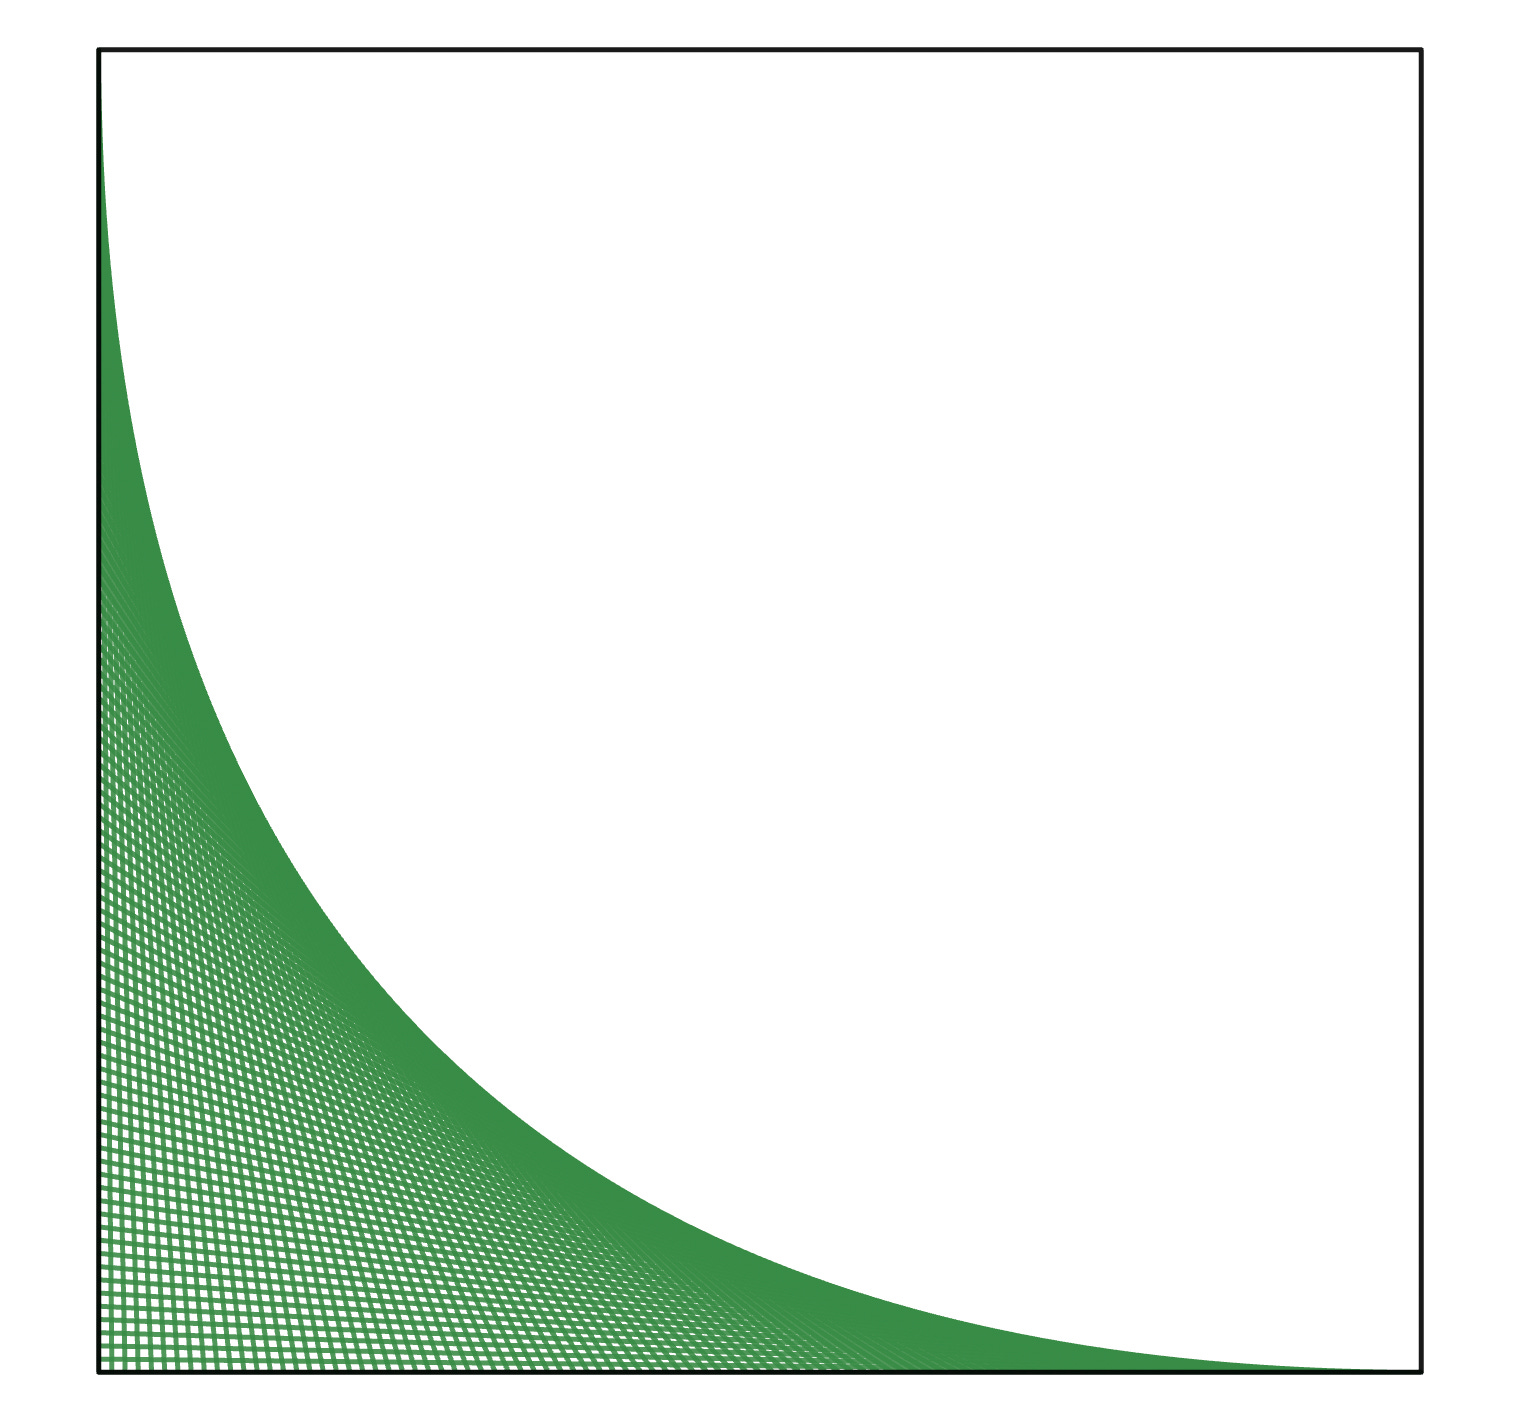
\includegraphics[width=0.7\textwidth]{Loom}
\end{figure}

As N increases, what is the shape of the curve formed by the edges of the bands? Your answer can be a single word or a mathematical equation.\\

\textbf{Solution}:\\
Suppose that the square has side length 1 with the bottom left corner at the origin. The curve is made up of the set of lines connecting $(0, t)$ to $(1-t, 0)$, where $t$ varies between 0 and 1. The idea is to fix one of these lines (the one with parameter $t$) and determine which point along the line is actually on the curve. This is done by finding the intersection point between the line with parameter $t$ and the line with parameter $t + h$, and taking the limit as $h$ goes to 0.\\

The equation for the line through $(t, 0)$ and $(0, 1-t)$ is given by:
\begin{equation}
\label{eq:line_t}
(1-t)x + ty = (1-t)t.
\end{equation}

Similarly, the equation of the line through $(t+h, 0)$ and $(0, 1-t-h)$ is given by:
\begin{equation}
\label{eq:line_th}
(1-t-h)x + (t+h)y = (1-t-h)(t+h).
\end{equation}

The intersection of these lines satisfies:
\begin{equation}
\label{eq:int_prob}
\left[\begin{array}{cc}
1-t & t\\1-t-h & t+h
\end{array}\right]
\left[\begin{array}{c}
x\\y
\end{array}\right]
=
\left[\begin{array}{c}
(1-t)t\\(1-t-h)(t+h)
\end{array}\right],
\end{equation}

which yields the solution
\begin{equation}
\label{eq:int_sol}
\left[\begin{array}{c}
x\\y
\end{array}\right]
=
\frac{1}{h}\left[\begin{array}{c}
ht(t+h)\\
h(1-t)(1-t-h)
\end{array}\right].
\end{equation}

In the limit as $h \rightarrow 0$, this converges to $(t^2, (1-t)^2)$. Therefore, the points along the curve satisfy $\sqrt{x} + \sqrt{y} = \sqrt{t^2} + \sqrt{(1-t)^2} = t + (1-t) = 1$.

Re-arranging, one obtains:
\begin{eqnarray*}
\sqrt{x} + \sqrt{y} & = & 1\\
y & = & (1-\sqrt{x})^2\\
y & = & 1 + x - 2\sqrt{x}\\
4x & = & (1 + x - y)^2\\
x^2 - 2xy + y^2 - 2x - 2y + 1 & = & 0.
\end{eqnarray*}

This has the form $Ax^2 + Bxy + Cy^2 + Dx + Ey + F = 0$, which is the equation of a conic section. Furthermore, $B^2 - 4AC = 0 $, so that this is the equation of a parabola.

\pagebreak

\textbf{Extra Credit Problem Statement}:\\
Let’s quadruple the number of bands placed on the weaving loom. In addition to the band connecting A1 and B1, you also place bands connecting B1 and C1, C1 and D1, and D1 and A1. You do this for all the sets of hooks from 1 through N, so that a total of 4N bands have been placed.\\

When N is 100, here is what the loom looks like:\\
\begin{figure}[h!]
\centering

\includegraphics[width=0.9\textwidth]{Loom2}
\end{figure}

As N increases, what fraction of the loom’s area lies between the four sets of bands? In other words, what fraction of the square above does the central white region make up?\\

\textbf{Solution}:\\
To make things easier, we'll compute the area of the central white region that is in the lower left quadrant of the square, where $(x, y) \in [0, 1/2]\times[0, 1/2]$. The leftmost point of the central white region is the value of $x$ where $\sqrt{x} + \sqrt{1/2} = 1$, which is $x = (1-\sqrt{2}/2)^2 = 3/2-\sqrt{2}$.\\

Therefore, the area we're looking for is bounded above by $y = 1/2$ and below by $y = (1-\sqrt{x})^2$, with x in the range $[3/2-\sqrt{2}, 1/2]$. This gives the integral:
\begin{equation}
\label{eq:integral}
\int_{3/2-\sqrt{2}}^{1/2}\left(\frac{1}{2} - (1-\sqrt{x})^2\right)dx.
\end{equation}

Evaluating this integral gives $2\sqrt{2}/3 - 5/6$, so that the full area is four times this, or $8\sqrt{2}/3 - 10/3 \approx 0.438$.

\end{document}